
\subsection{Présentation}

\frame{
\frametitle{Principaux objectifs (1)}

\begin{itemize}
\item Mise à jour / amélioration de ``l'utilisabilité'' des outils de la plateforme Ogmios/Alvis
\begin{itemize}
\item {\bf TreeTagger, YaTeA}
\item permettre utilisation en ``boîte noire''
\end{itemize}
\end{itemize}
\begin{itemize}
\item Jeter les bases d'une plateforme UIMA dédiée aux tâches étudiées par l'équipe (annotation sémantique)
\begin{itemize}
\item à long terme: améliorer la {\bf gestion/organisation des développements logiciels} de l'équipe
\item outils plus uniformes, compatibles, modulables, maintenace facilitée
\item {\bf évolutivité}
\end{itemize}
\end{itemize}
}


\frame{
\frametitle{Principaux objectifs (2)}

\begin{itemize}
\item Proposer une nouvelle approche dans la conception d'un {\em Type System}
\begin{itemize}
\item {\bf générique}: permettre/faciliter la composition de composants dans une chaîne
\begin{itemize}
\item transmission des données entre composants non homogènes
\end{itemize}
\item qui permet les {\bf annotations concurrentes}
\end{itemize}
\end{itemize}

Secondairement :
\begin{itemize}
\item Librairies ``utilitaires'' Java 

\item Possibilité de mise en place d'une politique de gestion logicielle
\begin{itemize}
\item ... si les intéressés le souhaitent bien sûr !
\end{itemize}
\end{itemize}
}

\frame{
\frametitle{UIMA en bref}

\begin{itemize}
\item un {\em Framework} pour ``encadrer'' l'analyse de grands volumes de données non structurées
\begin{itemize}
\item ``analyse'' $\approx$ découverte de connaissances ``utiles''
\item implémentation nettement orientée données textuelles
\end{itemize}
\item[$\rightarrow$] Ensemble d'{\bf outils} et (surtout) de {\bf conventions}
\begin{itemize}
\item But: partage, faciliter la communication inter-composants
\item Systèmes complexes avec composants indépendants mais composables
\item[$\Rightarrow$] Standardisation des composants + flexibilité
\end{itemize}
\item Implémentation Apache UIMA en {\bf Java}
\begin{itemize}
\item open-source, développement rapide
\end{itemize}
\end{itemize}
}



\frame{
\frametitle{Caractéristique: composants par encapsulation}


\begin{itemize}
\item Appel à un programme externe pour la réalisation de la tâche 
\item[$\rightarrow$] Avantage :  coût de développement moindre, outils connus
\item[$\rightarrow$] Inconvénients nombreux, non conforme à philosophie UIMA 
\begin{itemize}
\item portabilité $\searrow$ 
\item failles potentielles (entrées/sorties, gestion d'erreurs, multi-threading)
\item rupture du contrôle UIMA sur les composants
\begin{itemize}
\item conséquences sur chaîne complexe
\end{itemize}
\item perte d'efficacité temps/espace
\end{itemize}
\end{itemize}

\begin{itemize}
\item Gestion de ces problèmes
\begin{itemize}
\item Librairie d'appel ``protégé'' à un programme extérieur
\begin{itemize}
\item possibilité de lire/écrire à la volée
\end{itemize}
\item Librairie de (ré)-alignement, conversion entre formats
%\begin{itemize}
%\item modulable et paramétrable
%\end{itemize}
\end{itemize}
\end{itemize}
}


%\subsection{Contexte}

\frame{
\frametitle{Contexte}

\begin{itemize}
\item Projet Quaero
\begin{itemize}
\item WP 3.4 ``Développement d'une nouvelle plateforme d'annotation''
\end{itemize}
\item Casting :
\begin{itemize}
\item Maître d'\oe uvre : Laurent Audibert
\item Travail préliminaire par Sondes Bannour
\item Aide du LINA (Univ Nantes), notamment Fabien Poulard
\end{itemize}
\item Prototype quasi-``version beta'' {\small (phase tests utilisateurs)}
\begin{itemize}
\item Composants principaux terminés
\item Ajout des dernières fonctionnalités 
\item Documentation en cours de rédaction
\item {\em Release} version stable très bientôt
\end{itemize}
\end{itemize}
}


\frame[plain]{
%\frametitle{Une page de publicité}

\noindent\begin{center}
\noindent\scalebox{.37}[.37]{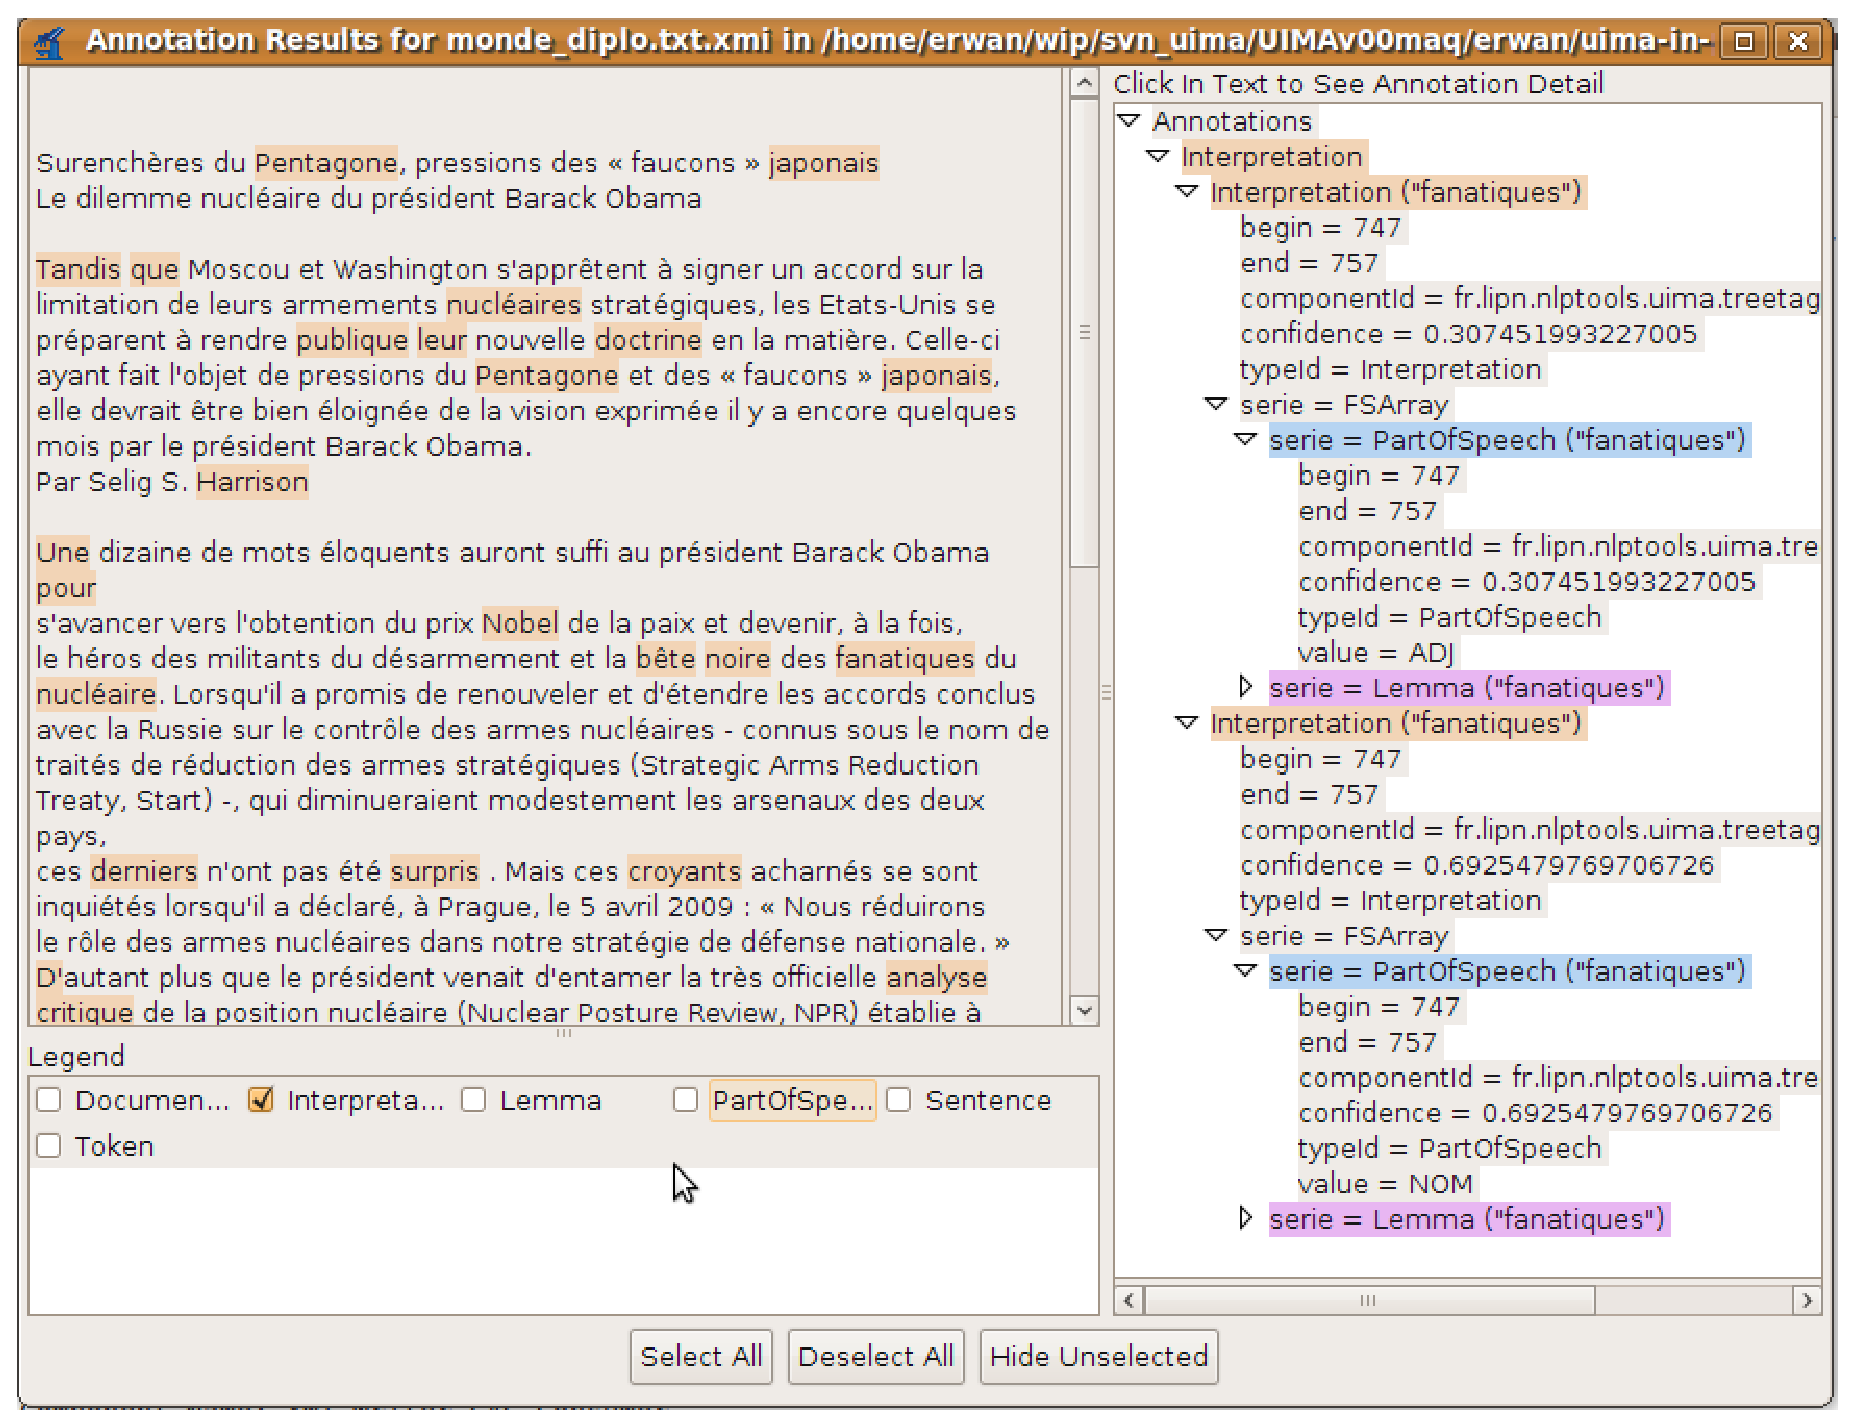
\includegraphics{capture_viewer_expl_interpretations.eps}}
\end{center}

}

\frame{
\frametitle{Plan}
\tableofcontents[hideallsubsections]

}

